\documentclass[letterpaper,11pt]{report}
% Change margins to 1 inch on all sides
\addtolength{\oddsidemargin}{-.875in}
\addtolength{\evensidemargin}{-.875in}
\addtolength{\textwidth}{1.75in}
\addtolength{\topmargin}{-.875in}
\addtolength{\textheight}{1.75in}
\usepackage{float}
\usepackage{graphicx}
\usepackage{footnote}
\usepackage{longtable}
\usepackage{multirow}
\usepackage{tablefootnote}
\usepackage{tabularx}
\usepackage{url}
\DeclareGraphicsExtensions{.pdf,.png,.jpg}

%%%%%%%%%%Start of report
\begin{document} 
\begin{savenotes}
\pagestyle{plain}
\title{CS896 Introduction to Web Science\\Fall 2013\\Report for Assignment 9}
\author{Corren G. McCoy}
 
\date{December 5, 2013}
\maketitle

\renewcommand*\thesection{\arabic{section}}
\setcounter{section}{0}

\setcounter{tocdepth}{4}
\tableofcontents
 \listoffigures
\newpage


%%%%%%%%%%Chapter Exercises
\section{Question 1}
\subsection{Problem}Create a blog-term matrix. Use the blog title as the identifier for each blog (and row of the matrix).  Use the terms from every item/title (RSS) or entry/title (Atom) for the columns of the matrix.  The values are the frequency of occurrence.  Essentially you are replicating the format of the ``blogdata.txt'' file included with the PCI book code.  Limit the number of terms to the most ``popular'' (i.e., frequent) 500 terms, this is *after* the criteria on p. 32 (slide 7) has been satisfied.
\begin{itemize}
\item \url{http://f-measure.blogspot.com/}
\item \url{http://ws-dl.blogspot.com/}
\end{itemize}

\subsection{Response}We will use the techniques described in Segaran \cite{segaran2007programming} to cluster a set of 100 blogs based on the number of times a particular word appears in the title of each blog. To generate the complete dataset needed for this problem, we used the two recommended blogs along with a pre-built, supplementary dataset provided with the textbook material. The supplementary dataset contains 100 RSS URLs which represent the ``feeds for all of the most highly referenced blogs'' according to Segaran. To facilitate clustering later, we randomly replaced approximately 25\% of the blogs in the supplementary dataset with blogs that represent sports (e.g., NFL, baseball), television and online news media, and technology. The modified Python function \emph{generatefeedvector.py}, shown in Appendix \ref{chap:python}, performs the following tasks.
\begin{itemize}
\item Parse the XML for the RSS or ATOM feed using the Universal Feed Parser (\url{http://code.google.com/p/feedparser/}).
\item Identify the blog entries using either the \emph{summary} or \emph{description} tag.
\item Strip the HTML and returns a list of words. Sort the list in descending order based on the frequency.
\item Eliminates common words based on a minimum and maximum frequency percentage (10 to 50\%) based on the accumulated word count in the feed list. We also applied a filter to ensure that only significant words, with a length of at least three characters, remain in the list.
\item Extract the 500 most popular terms from the word list.
\item Use the resulting list of words and the blog names to create the blog-term matrix (i.e.,blogdata.txt). The text file is included in the github supporting files for this assignment (\url{https://github.com/correnm/cs595-f13/tree/master/Supporting Files}.
\end{itemize}

%%%%%%%%%%Chapter Exercises
\section{Question 2}
\subsection{Problem}Create an ASCII and JPEG dendrogram that clusters (i.e., HAC) the most similar blogs (see slides 12 \& 13).  Include the JPEG in your report and upload the ascii file to github (it will be too unwieldy for inclusion in the report).

\subsection{Response}We slightly modified the \emph{clusters.py} found in Segaran \cite{segaran2007programming} to adjust the dimensions and redirect the output when producing the dendrogram. The updated source code is shown in Appendix \ref{chap:python}. The complete ASCII version, \emph{ascii-dendrogram.txt}, is included in the github supporting files for this assignment (\url{https://github.com/correnm/cs595-f13/tree/master/Supporting Files}. An example of the clusters around our two recommended URLs is shown below:

\begin{verbatim}
                   Washington Post: Breaking News, World, US, DC News \& Analysis
                   -
                     Web Science and Digital Libraries Research Group
                     -
                       Boing Boing
                       -
                         kottke.org
                         -
                           Gothamist
                           -
                             F-Measure
                             -
                                Wired Top Stories
                                Technology
\end{verbatim}
																									
As explained by Segaran, ``the dashes represent a cluster of two or more  merged  items.'' An examination of the ASCII dendrogram does, as expected, show definite clusters around the news and sport sites we placed in the feed list.  We also see a few of our news feeds clustered with other non-news groups which could be an anomaly or indicative of the stories present on the day these blogs were downloaded. In either case, the correlation is based on the word frequency in the blogs. The graphical version of the dendrogram is shown in Figure \ref{fig:blogclust}.

\begin{figure}
	\centering
		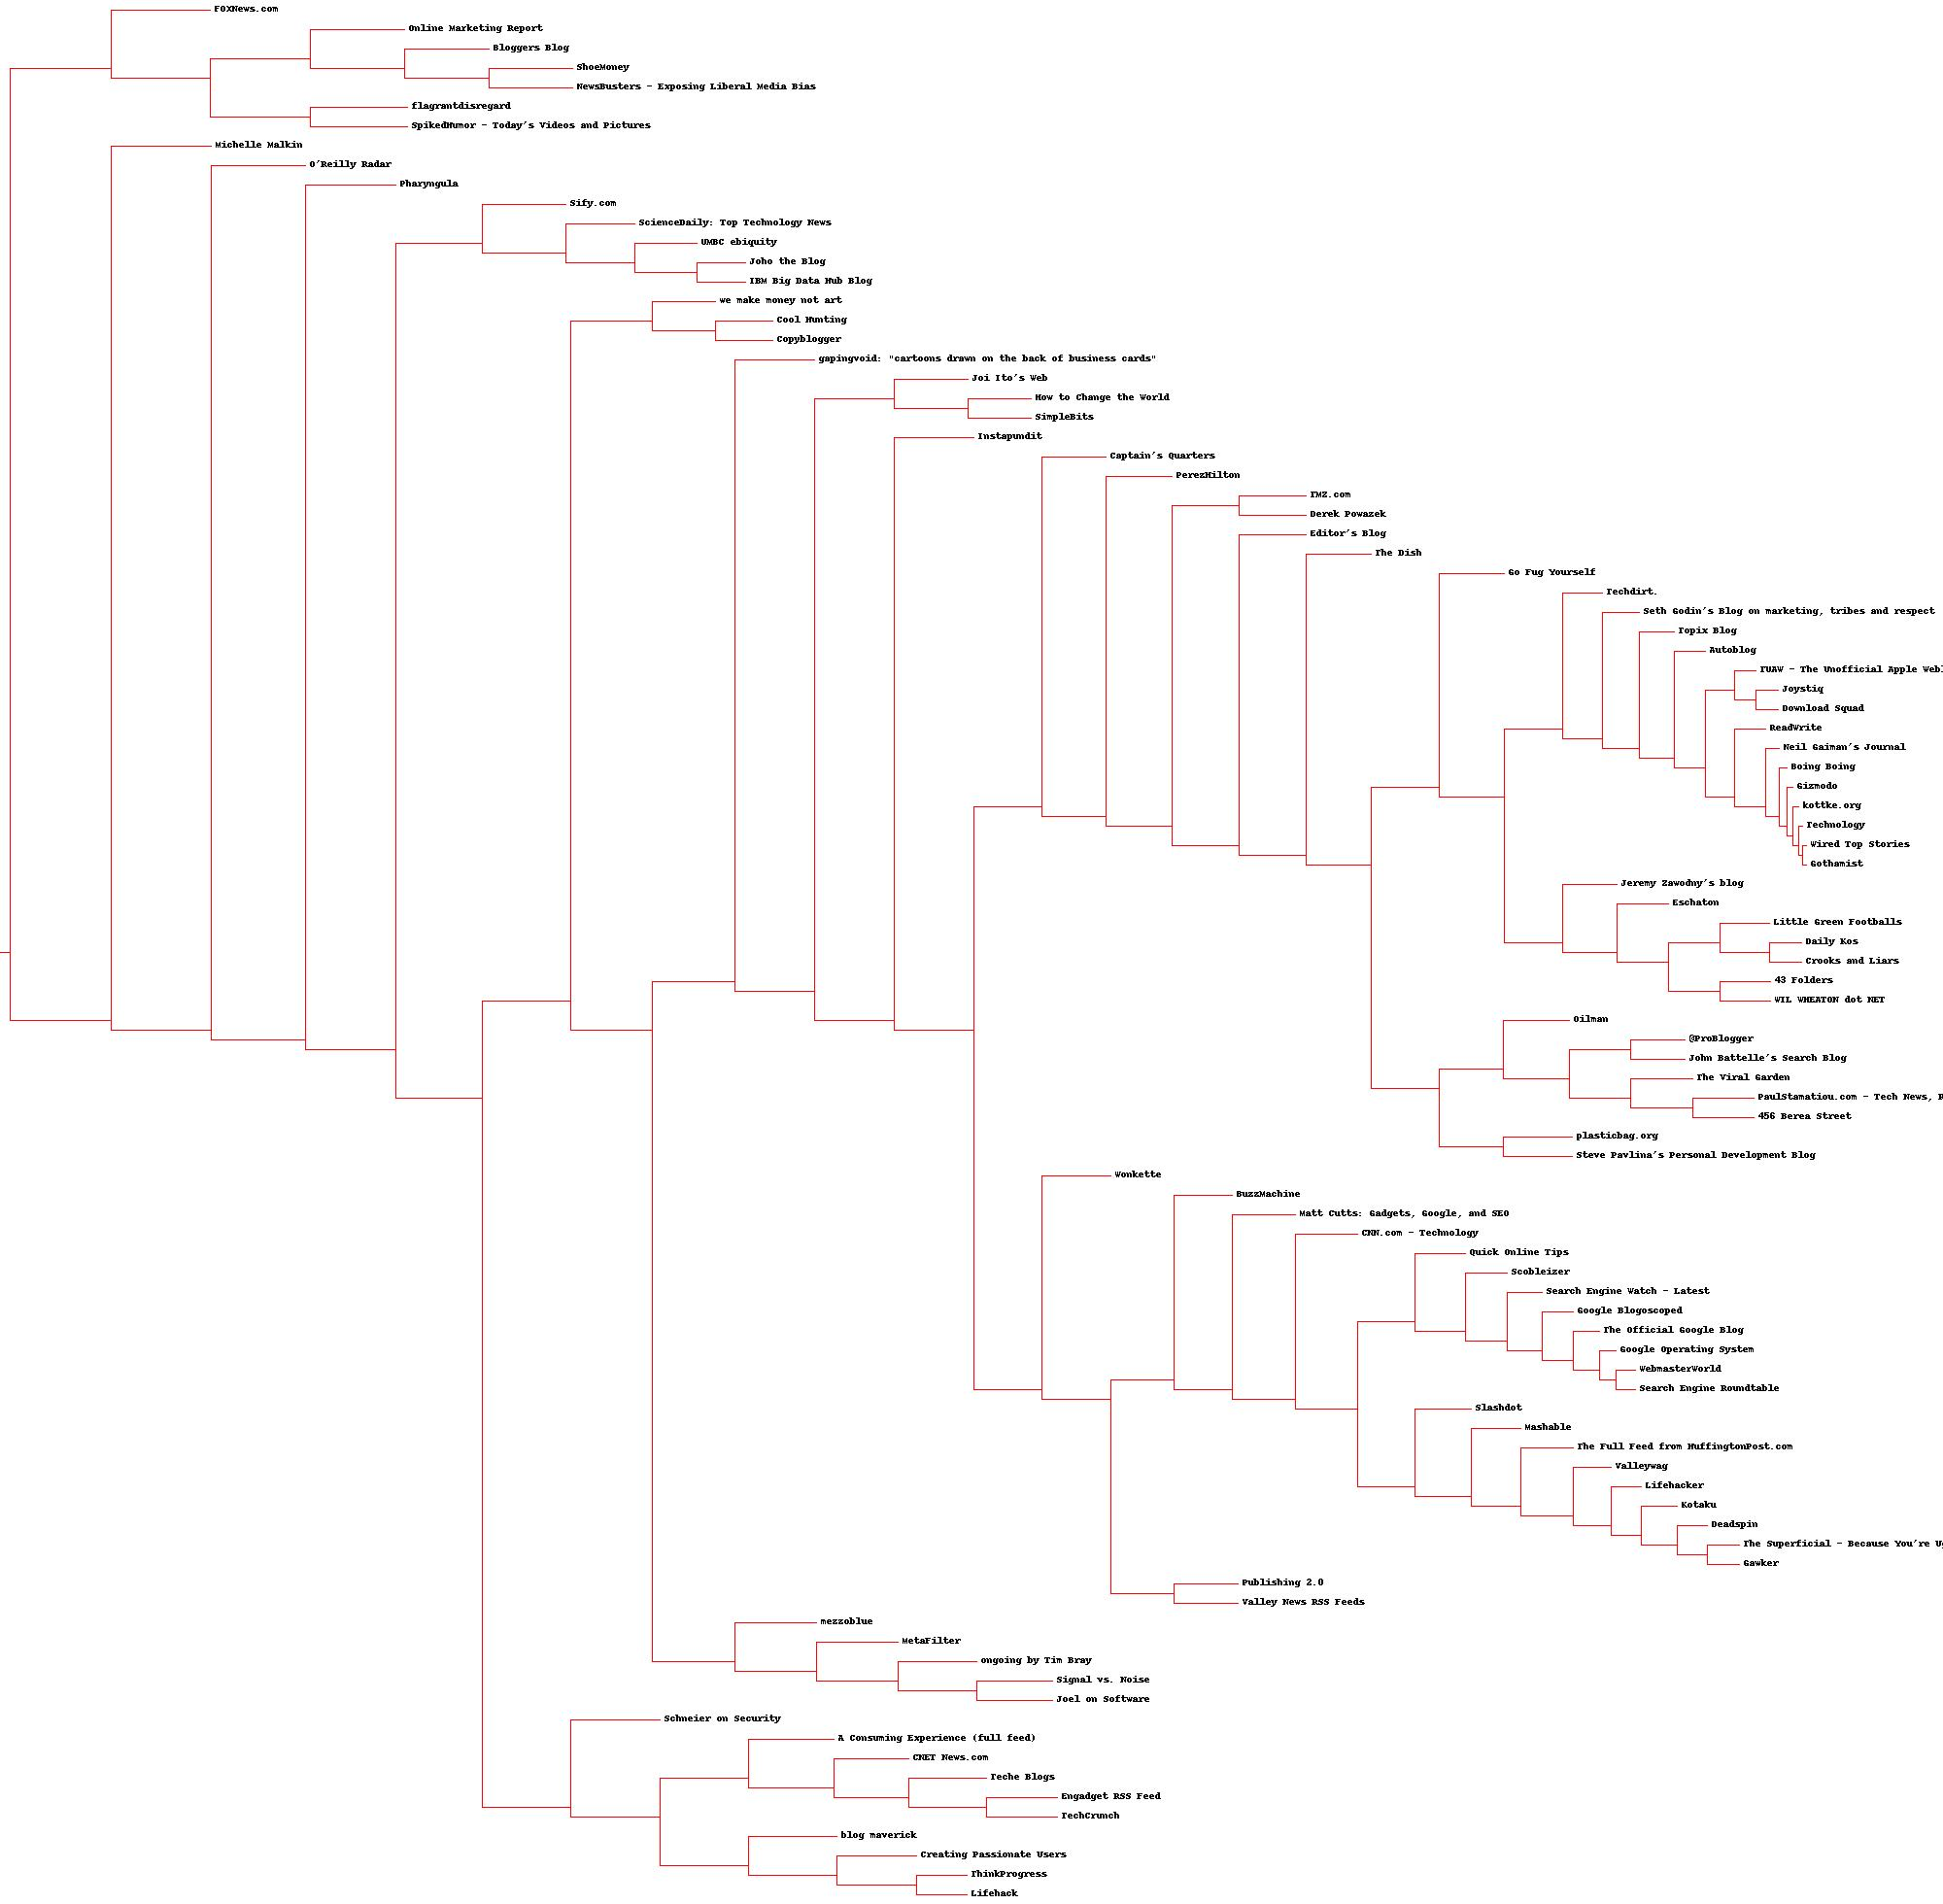
\includegraphics[width=1.00\textwidth]{blogclust.jpg}
	\caption{JPEG Dendrogram}
	\label{fig:blogclust}
\end{figure}

%%%%%%%%%%Chapter Exercises
\section{Question 3}
\subsection{Problem}Cluster the blogs using K-Means, using k=5, 10, 20. (see slide 18). How many interations were required for each value of k?
\subsection{Response}We used functions in \emph{clusters.py} to apply k-means to the hierarchical clusters for our set of blogs. We obtained the following results using various values for the number of desired clusters. We did note variations in the number of iterations required on subsequent executions of the same algorithm. Croft \cite{croft2010search} provides one possible explanation for this observation which is the naive assignment of items to an initial cluster. To obtain more consistent results would require that we remove the element of randomness and instead use some knowledge of the data to make a better decision.

\begin{itemize}
\item When k=5, iterations=3
\item When k=10, iterations=6
\item When k=20, iterations=5
\end{itemize}

%%%%%%%%%%Chapter Exercises
\section{Question 4}
\subsection{Problem}Use MDS to create a JPEG of the blogs similar to slide 29.  How many iterations were required?

\subsection{Response}We used functions in \emph{clusters.py} to apply the multidimensional scaling (MDS) algorithm. 175 iterations were required to produce the JPEG shown in Figure \ref{fig:blogs2d}. This visual representation should be easier to interpret than a dendrogram. As previously noted during hierarchical clustering, we see a grouping of news sites near the top of diagram which are considerably distanced from the technology blogs near the bottom. The distance is indicative of the perceived dissimilarity. We also notice several blogs which appear to be so similar, based on distance, that the titles overlap. Two of these blogs are \emph{Wired Top Stories} and \emph{Web Science and Digital Library Research Group}. In close proximity is another pair of titles which are seated directly on top of one another, \emph{Kottke} and \emph{Gothamist Daily}, both sites have blog entries that discuss pop culture happenings in and around New York City. The same relationships were observed in the clustering of our ASCII dendrogram.

\begin{figure}[htbp]
	\centering
		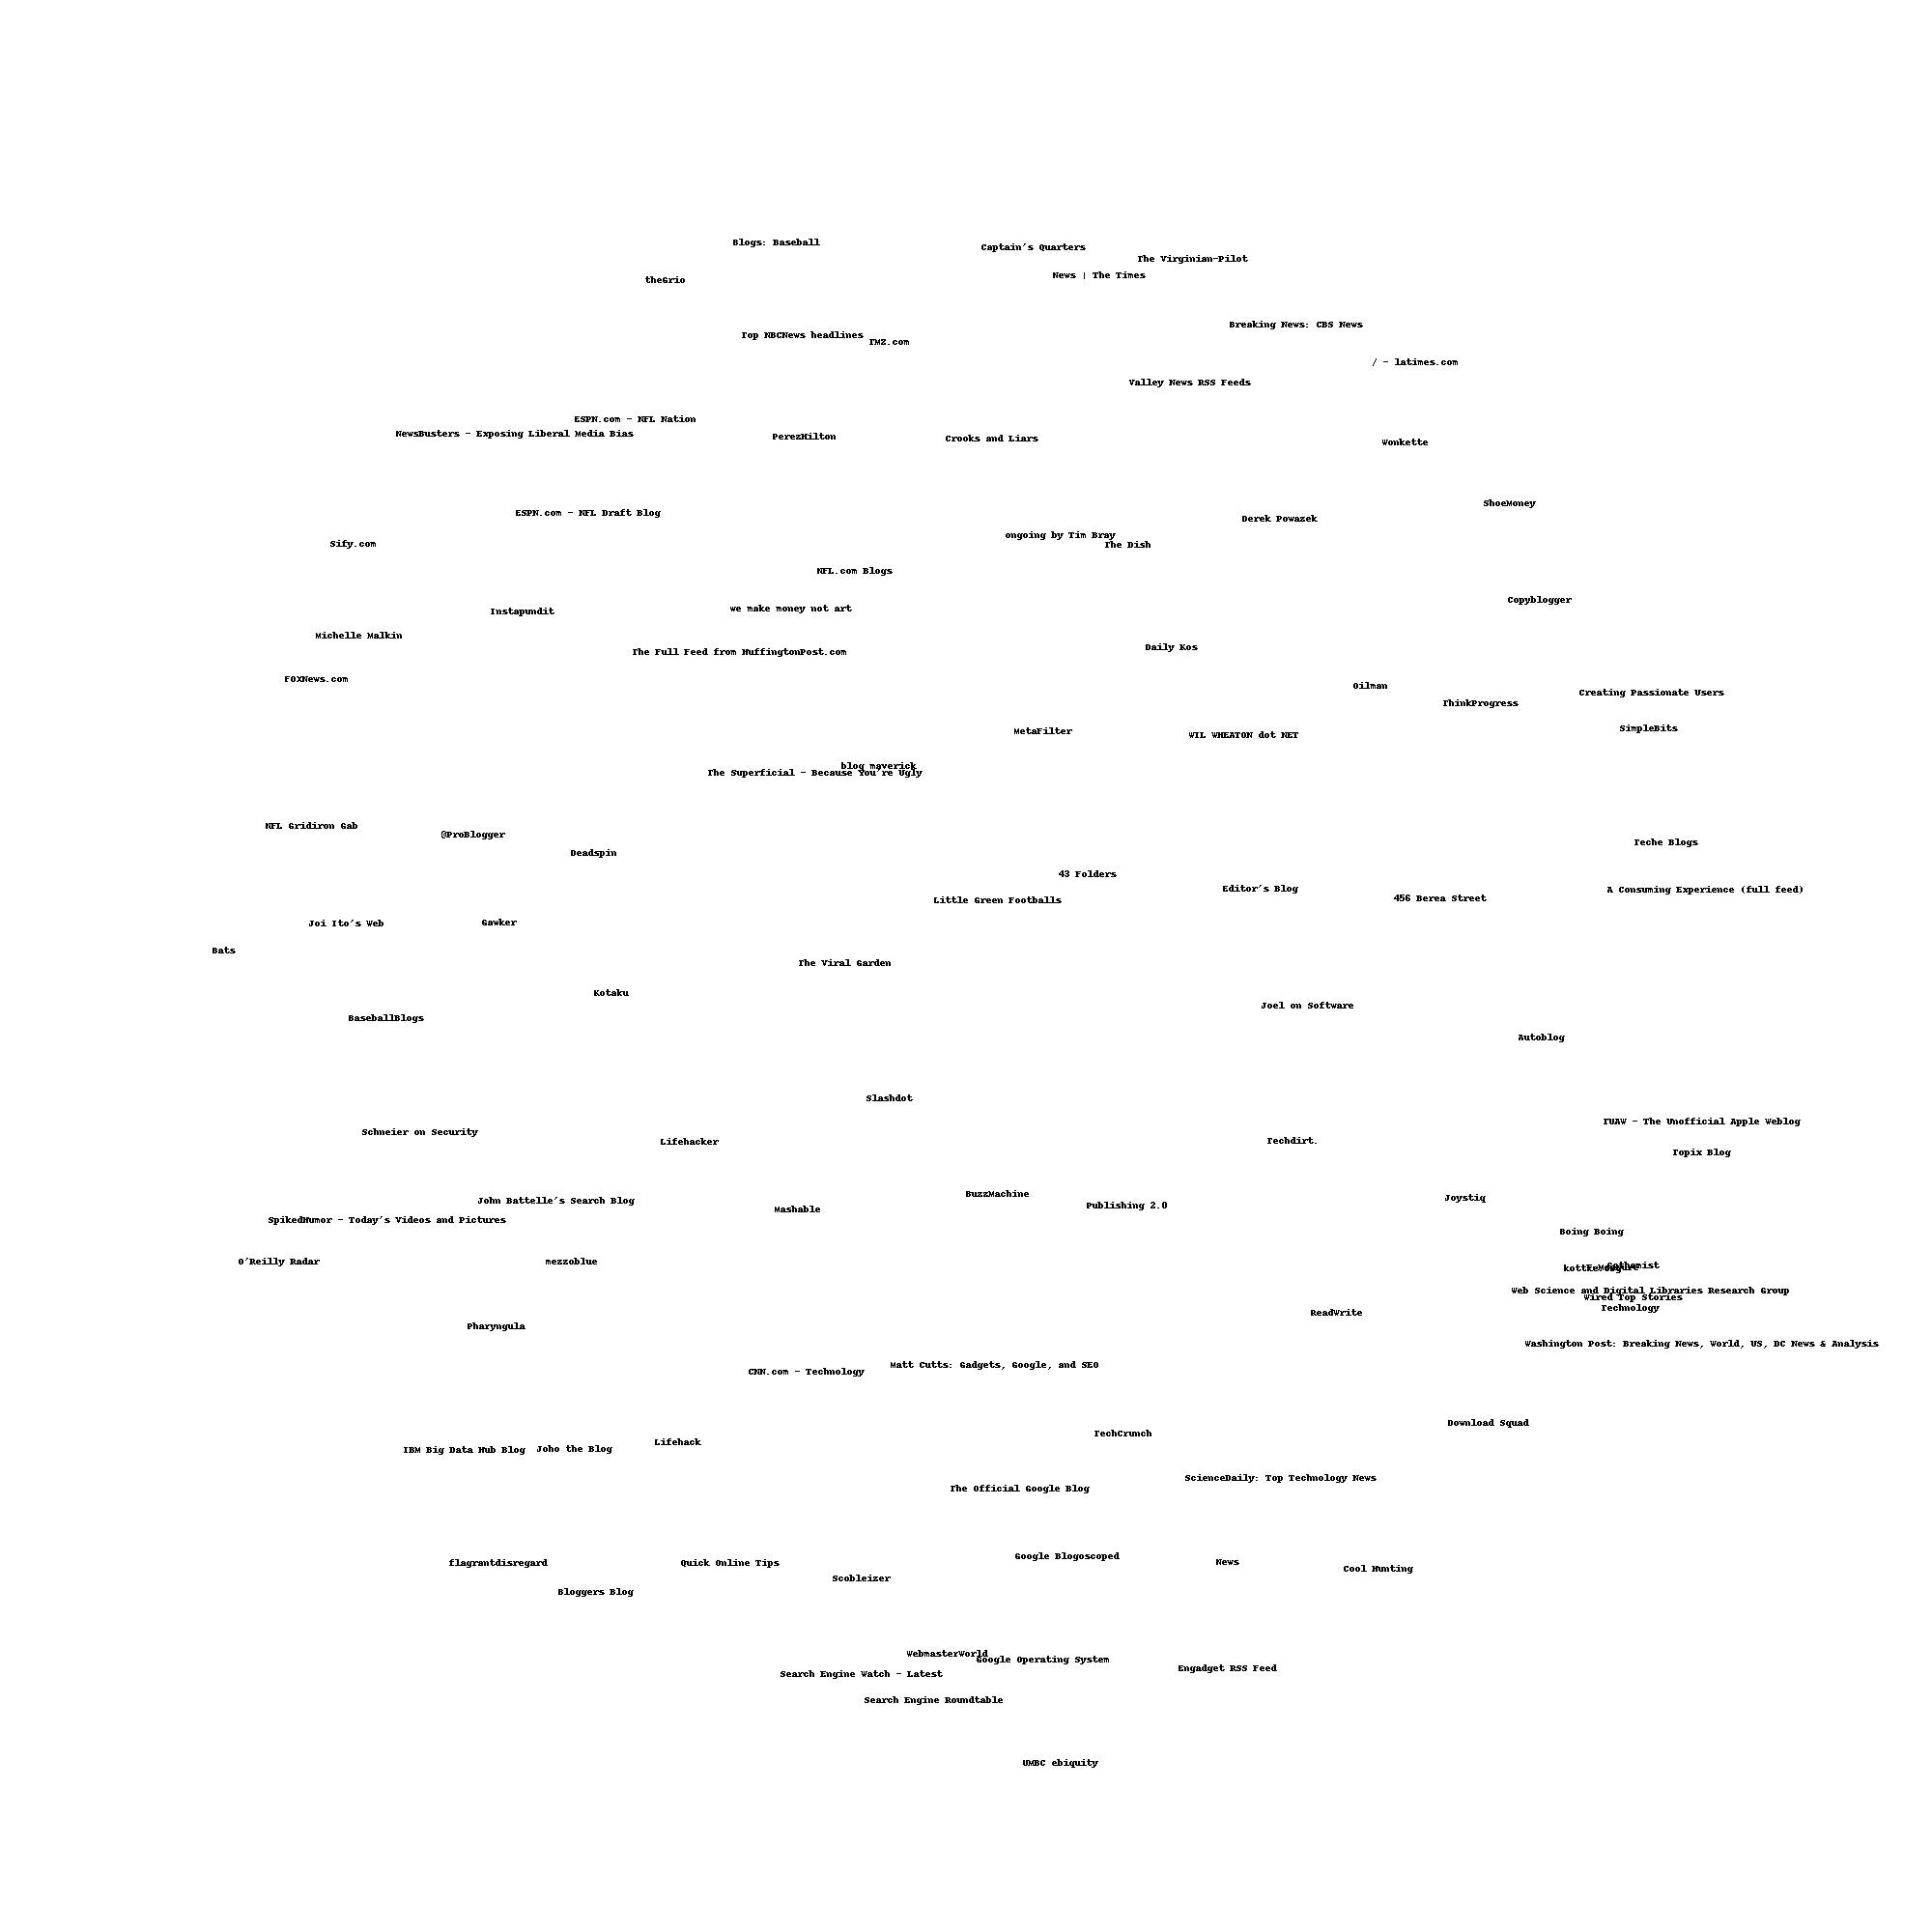
\includegraphics[width=1.00\textwidth]{blogs2d.jpg}
	\caption{MDS for Blogs}
	\label{fig:blogs2d}
\end{figure}

\section{Question 5 Extra Credit}
\subsection{Problem}Re-run question 2, but this time with proper TFIDF calculations instead of the hack discussed on slide 7 (p. 32).  Use the same 500 words, but this time replace their frequency count with TFIDF scores as computed in assignment \#3.  Document the code, techniques, methods, etc. used to generate these TFIDF values.  Upload the new data file to github. Compare and contrast the resulting dendrogram with the dendrogram from question \#2.
\subsection{Response}Not attempted.

\end{savenotes}

% produce the bibliography for the citations in your paper.
\bibliographystyle{abbrv}
\bibliography{cmccoy}

\appendix
\addcontentsline{toc}{chapter}{Appendices}

%%Appendix A
\chapter{Python Source Code} \label{chap:python}
\input{generatefeedvector.py}
\input{clusters.py}


\end{document} 
%%%%%%%%%%Ed of report
